\subsection{Schemat}
	\begin{center}
		\begin{figure}[h!]
			\makebox[\textwidth]{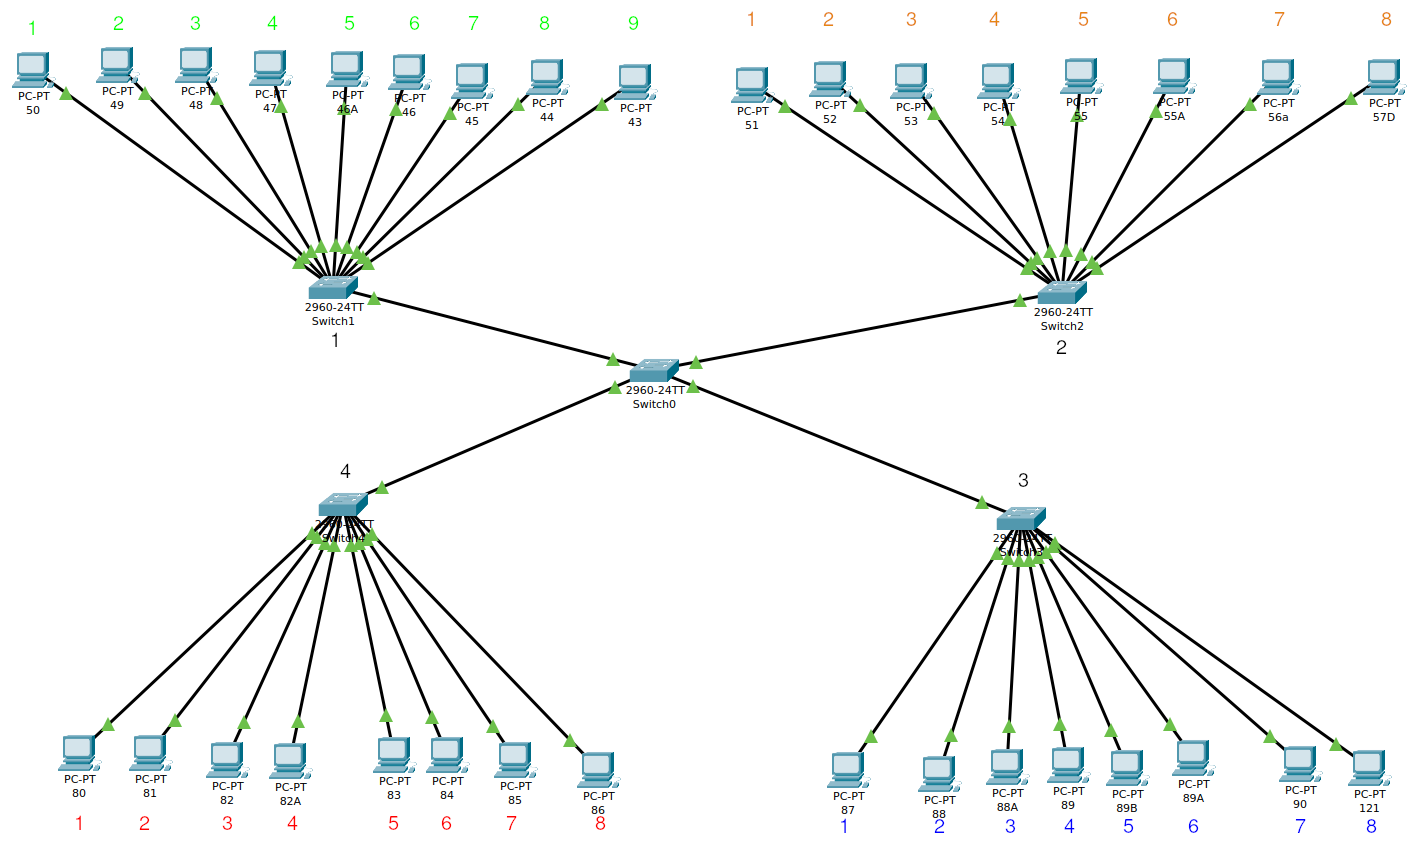
\includegraphics[width=\textwidth]{schemat_logiczny.png}}
			\caption{Schemat logiczny}
			\label{fig:schemat_logiczny}
		\end{figure}
		\begin{figure}[h!]
			\makebox[\textwidth]{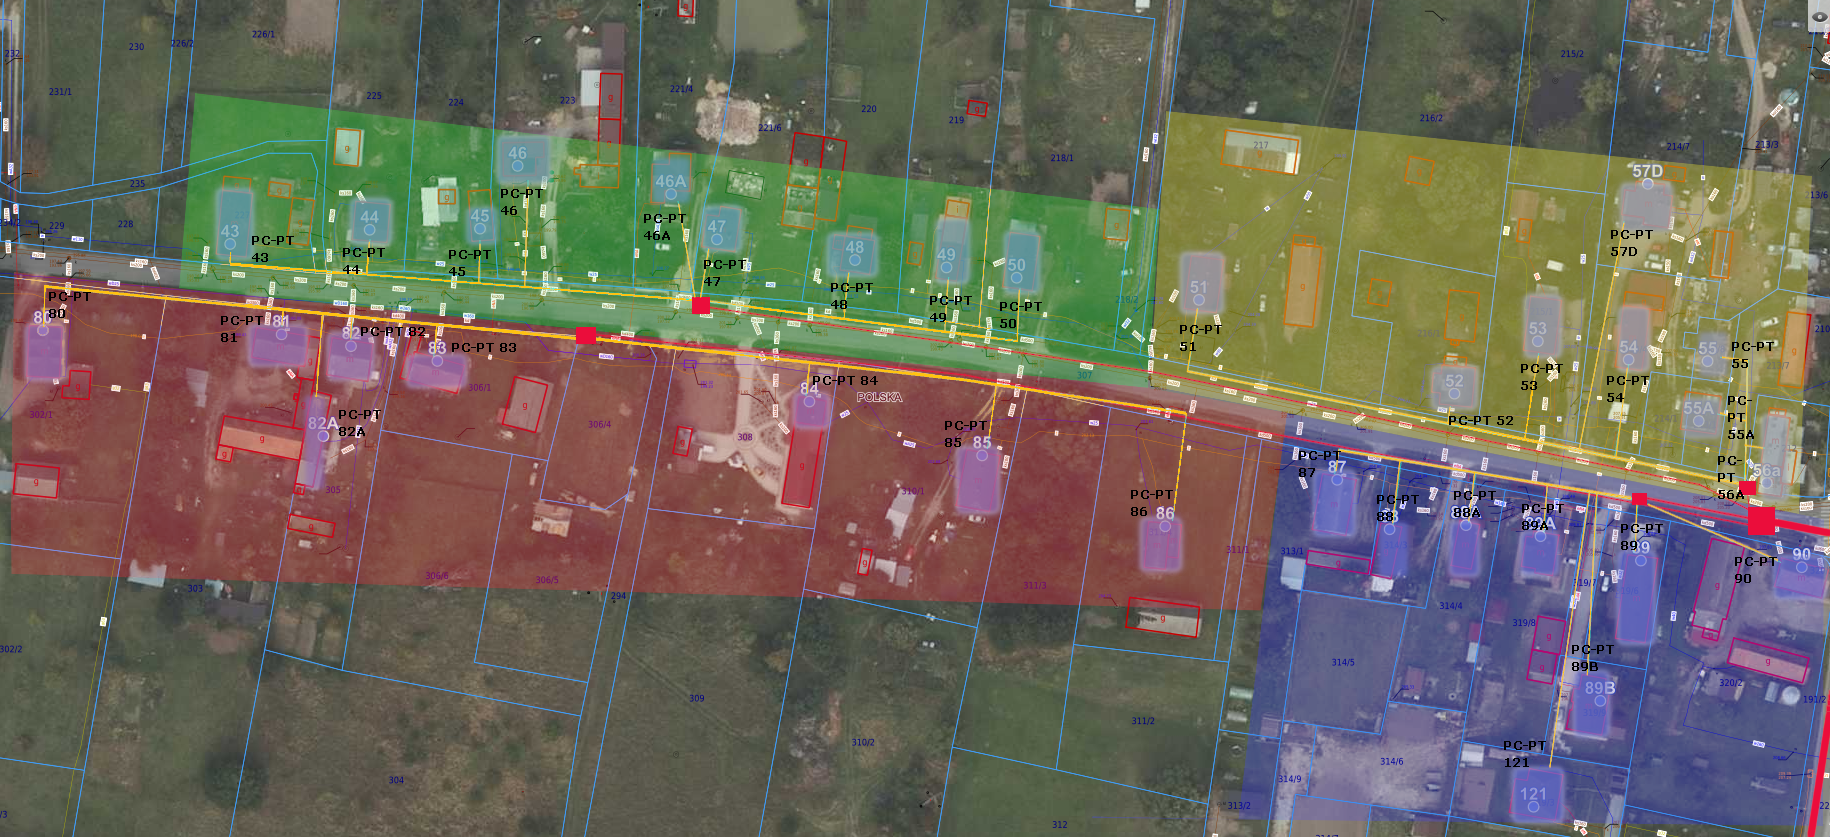
\includegraphics[width=\textwidth]{proj_gimp/proj.png}}
			\caption{Podział na podsieci na mapie fizycznej}
			\label{fig:podsieci}
		\end{figure}
	\end{center}

\subsection{Rozwiązania techologiczne}
	\paragraph{Okablowanie:}
		SM G657
	\paragraph{Złącza:}
		SC/APC (Subscriber Connector)
	\paragraph{Użyte sprzęgacze:}
		\begin{center}
			\begin{table}[htbp]
				\centering
				\begin{tabular}{|c|c|}
					\hline
					\textbf{Typ} & \textbf{ilość} \\ \hline
					1x4          & 1              \\ \hline
					1x16         & 4              \\ \hline
				\end{tabular}
			\end{table}
		\end{center}
\subsection{Podział na podsieci}
	\begin{center}
		\begin{table}[htbp]
			\centering
			\begin{tblr}{
					cells = {BrightTurquoise},
					row{2} = {c},
					column{1} = {Green},
					column{2} = {Green},
					column{3} = {Turbo},
					column{4} = {Turbo},
					column{7} = {Persimmon},
					column{8} = {Persimmon},
					cell{1}{1} = {c=2}{c},
					cell{1}{3} = {c=2}{},
					cell{1}{5} = {c=2}{},
					cell{1}{7} = {c=2}{},
					cell{3}{1} = {c},
					cell{3}{2} = {c},
					cell{4}{1} = {c},
					cell{4}{2} = {c},
					cell{5}{1} = {c},
					cell{5}{2} = {c},
					cell{6}{1} = {c},
					cell{6}{2} = {c},
					cell{7}{1} = {c},
					cell{7}{2} = {c},
					cell{8}{1} = {c},
					cell{8}{2} = {c},
					cell{9}{1} = {c},
					cell{9}{2} = {c},
					cell{10}{1} = {c},
					cell{10}{2} = {c},
					cell{11}{1} = {c},
					cell{11}{2} = {c},
					hlines,
					vlines,
				}
				\textbf{Podsieć 1} &      & \textbf{Podsieć 2} &      & \textbf{Podsieć 3} &      & \textbf{Podsieć 4} &      \\
				nr działki         & port & nr działki         & port & nr działki         & port & nr działki         & port \\
				43                 & 9    & 51                 & 1    & 87                 & 1    & 80                 & 1    \\
				44                 & 8    & 52                 & 2    & 88                 & 2    & 81                 & 2    \\
				45                 & 7    & 53                 & 3    & 88A                & 3    & 82                 & 3    \\
				46                 & 6    & 54                 & 4    & 89                 & 4    & 82A                & 4    \\
				46A                & 5    & 55                 & 5    & 89A                & 6    & 83                 & 5    \\
				47                 & 4    & 55A                & 6    & 89B                & 5    & 84                 & 6    \\
				48                 & 3    & 56A                & 7    & 90                 & 7    & 85                 & 7    \\
				49                 & 2    & 57D                & 8    & 121                & 8    & 86                 & 8    \\
				50                 & 1    &                    &      &                    &      &                    &      
			\end{tblr}
		\end{table}
	\end{center}